% Supported aspectratio 43|169, default is 43
\documentclass[aspectratio=169]{beamer}
\usetheme[theme=blue,logo=logowithtextvi]{HUST} % <-- this matches beamerthemeHUST.sty

% \usepackage[utf8]{vietnam}
\usepackage[T5]{fontenc}
% \setmainfont{assets/fonts/LATO-BLACK.TTF}
\usepackage{enumitem}
\usepackage{tcolorbox}
\usepackage{listings}
\usepackage{verbatim}
\usepackage{amsmath}
\usepackage[table]{xcolor}
\usepackage{tikz}
\usetikzlibrary{decorations.pathreplacing,arrows.meta}


\tcbuselibrary{listingsutf8}




\newcommand{\placecontent}[4]{%
  \tikz[remember picture,overlay]
    \node[anchor=north west]
      at ([xshift=#1,yshift=-#2]current page.north west)
      {\parbox{#3}{#4}};
}


\title{CẤU TRÚC DỮ LIỆU VÀ THUẬT TOÁN}
\author{SoICT - HUST}
\date{}
\setbeamertemplate{footline}{%
  \hfill%
  \insertframenumber\hspace{0.5cm}\vspace{0.3cm}
  }
\begin{document}

\HUSTInsertBrandSlide
\HUSTInsertThemeSlide

% Title slide - place it here for your customization
{\HUSTUseBackground{onelove.pdf}
\begin{frame}
  \ifdefstring{\insertaspectratio}{169}{
    \HUSTCornerImage{assets/logo/04.pdf}

    %----------You can edit here----------
    \placecontent{0.5cm}{0.33\paperheight}{0.85\paperwidth}{
        \color{\HUSTFrameTitleTextColor}\bfseries\fontsize{22pt}{30pt}\selectfont
        \inserttitle
    }
    % \placecontent{0.5cm}{0.48\paperheight}{10cm}{    % one-line title
    \placecontent{0.5cm}{0.60\paperheight}{0.5\paperwidth}{    % two-line title
        \color{\HUSTFrameTitleTextColor}\fontsize{12pt}{14pt}\selectfont
        TUẦN 1 : CÁC KHÁI NIỆM CƠ BẢN\\
        \insertauthor
    }
  }{}
  \ifdefstring{\insertaspectratio}{43}{
    \HUSTCornerImage[0.1][0.35cm][-0.03]{assets/logo/04.pdf}

    %----------You can edit here----------
    \placecontent{0.5cm}{0.33\paperheight}{0.80\paperwidth}{
        \color{\HUSTFrameTitleTextColor}\bfseries\fontsize{18pt}{22pt}\selectfont
        \inserttitle
    }
    % \placecontent{0.5cm}{0.48\paperheight}{10cm}{    % one-line title
    \placecontent{0.5cm}{0.60\paperheight}{0.5\paperwidth}{    % two-line title
        \color{\HUSTFrameTitleTextColor}\fontsize{12pt}{14pt}\selectfont
        TUẦN 1 : CÁC KHÁI NIỆM CƠ BẢN\\
        \insertauthor
    }
  }{}
\end{frame}
}

% Display the tableofcontents before a section
\AtBeginSection[]
{
    \begin{frame}<beamer>
        \frametitle{MỤC LỤC}
        \tableofcontents[currentsection]
    \end{frame}
}

%Phần này không cần chỉnh theo tỉ lệ slide 43 69 "
\begin{frame}{MỤC TIÊU}
    \hspace{1.5cm}\textit{\color{HUSTBlue}Sau bài học này, người học có thể:}\vspace{0.5cm}

    \begin{itemize}
        \item 1. Hiểu được một số \textcolor{HUSTRed}{khái niệm cơ bản về thuật toán}
        \item 2. Biết \textcolor{HUSTRed}{ký hiệu tiệm cận} dùng để đánh giá độ phức tạp thuật toán
        \item 3. Biết cách \textcolor{HUSTRed}{phân tích độ phức tạp của thuật toán}
    \end{itemize}
  
\end{frame}

%slide 1 section 1
\section{Ví dụ minh họa}
\begin{frame}{1. Ví dụ minh họa}
  \begin{itemize}[label={\tiny$\blacksquare$}] 
    \item {\color{HUSTBlue}Bài toán tìm dãy con lớn nhất:}
      \begin{itemize}[label={\tiny$\bullet$}]
        \item Cho dãy số gồm $n$ số: $a_0, a_1, a_2, ..., a_{n-1}$

        \item Dãy gồm liên tiếp các số $a_i, a_{i+1},\ldots,a_j$ với $0 \leq i \leq j \leq n-1$ được gọi là 
          \textcolor{HUSTYellow}{dãy con} của dãy đã cho và $\sum_{k=i}^j a_k$ được gọi là trọng lượng của dãy con này
        \item \color{HUSTYellow}\textbf{Hãy tìm trọng lượng lớn nhất của dãy con, tức là tìm cực đại giá trị} $\sum_{k=i}^j a_k$ . Ta gọi dãy con có trọng lượng lớn nhất là \textbf{dãy con lớn nhất.}
    \end{itemize}
    \pause
  \item \textbf{Ví dụ:} Cho dãy số $-2, \textcolor{HUSTYellow}{11, -4, 13}, -5, 2$ thì cần đưa ra câu trả lời là 20 (dãy con lớn nhất là 11, -4, 13 với giá trị $= 11 + (-4) + 13 = 20$)
\end{itemize}

\end{frame}
% "

%slide 2 section 1

\begin{frame}[fragile]{1. Ví dụ minh họa}
  \begin{itemize}[label={\tiny$\blacksquare$}]
    \item {\color{HUSTBlue}Cách 1: Duyệt toàn bộ}
      \begin{itemize}[label={\tiny$\bullet$}]
        \item Duyệt tất cả các dãy con có thể có của dãy đã cho:
          \textcolor{HUSTYellow}{$a_i, a_{i+1},\ldots,a_j$ với $0 \leq i \leq j \leq n-1$,}
          và tính tổng của mỗi dãy con để tìm ra trọng lượng lớn nhất.
      \end{itemize}
  \end{itemize}
% code C in box


\vspace{0.5em}

\begin{center}
\begin{tcolorbox}[colback=gray!10, colframe=black,boxrule=1pt,
    width=0.6\textwidth]
\scriptsize
\begin{lstlisting}[language=C, basicstyle=\ttfamily\scriptsize\color{HUSTBlue}, breaklines=true]
int maxSum = a[0];
for (int i = 0; i <= n-1; i++) {
    for (int j = i; j <= n-1; j++) {
        int sum = 0;
        for (int k = i; k <= j; k++)
            sum += a[k];
        if (sum > maxSum) maxSum = sum;
    }
}
\end{lstlisting}
\end{tcolorbox}
\end{center}
\end{frame}


%slide 3 section 1
\begin{frame}[fragile]{1. Ví dụ minh họa}
\begin{itemize}
    \item Cách 1: Duyệt toàn bộ
    \begin{itemize}
        \item Duyệt tất cả các dãy con có thể có của dãy đã cho: $a_i, a_{i+1}, ..., a_j$ với $0 \leq i \leq j \leq n-1$, và tính tổng của mỗi dãy con để tìm ra trọng lượng lớn nhất.
        \item \textbf{Phân tích thuật toán:} Ta sẽ tính số lượng phép cộng mà thuật toán phải thực hiện, tức là đếm xem dòng lệnh \texttt{\textcolor{HUSTYellow}{sum += a[k]}} phải thực hiện bao nhiêu lần. Số lượng phép cộng là:
    \end{itemize}
\end{itemize}

%columns

\begin{columns}[T,onlytextwidth]
    \begin{column}{0.45\textwidth}
        \begin{tcolorbox}[colback=gray!10, colframe=black, boxsep=0.1pt, left=0.1pt, right=0.1pt, top=0.1pt, bottom=0.1pt]
            \tiny
\begin{lstlisting}[language=C, basicstyle=\ttfamily\tiny\color{HUSTBlue}, breaklines=true,escapeinside={(*@}{@*)} ]
int maxSum = a[0];
for (int i = 0; i<=n-1; i++) {
  for (int j = i; j<=n-1; j++) {
    int sum = 0;
    for (int k=i; k<=j; k++) (*@\textcolor{HUSTRed}{sum += a[k];}@*)
    if (sum > maxSum) maxSum = sum;
  }
}
\end{lstlisting}
        \end{tcolorbox}
    \end{column}

\hspace{0.5em}
    \begin{column}{0.55\textwidth}
        \tiny
        \begin{align*}
    &\sum_{i=0}^{n-1} \sum_{j=i}^{n-1} (j-i+1)
    = \sum_{i=0}^{n-1} \left( 1 + 2 + \cdots + (n-i) \right)
    = \sum_{i=0}^{n-1} \frac{(n-i)(n-i+1)}{2} \\
    &= \frac{1}{2} \sum_{k=1}^n k(k+1)
    = \frac{1}{2} \left[ \sum_{k=1}^n k^2 + \sum_{k=1}^n k \right] 
    = \frac{1}{2} \left[ \frac{n(n+1)(2n+1)}{6} + \frac{n(n+1)}{2} \right] \\
    &= \frac{n^3}{6} + \frac{n^2}{2} + \frac{n}{3}
\end{align*}
    \end{column}

\end{columns}
\end{frame}

%slide 4 section 1
\begin{frame}{1. Ví dụ minh họa}
  \begin{itemize}[label={\tiny$\blacksquare$}]
    \item {\color{HUSTBlue}Cách 2: Duyệt toàn bộ có cải tiến:}
    
    \begin{center}
    \renewcommand{\arraystretch}{1.3}
    \begin{tabular}{>{\raggedright\arraybackslash}p{1.6cm} 
                    >{\centering\arraybackslash}p{1cm} 
                    >{\centering\arraybackslash}p{1cm} 
                    >{\centering\arraybackslash}p{1cm} 
                    >{\centering\arraybackslash}p{1cm} 
                    >{\centering\arraybackslash}p{1cm} 
                    >{\centering\arraybackslash}p{1cm}}
         \rowcolor{orange!80}
        \textcolor{white}{Index i} & \textcolor{white}{0} & \textcolor{white}{1} & \textcolor{white}{2} & \textcolor{white}{3} & \textcolor{white}{4} & \textcolor{white}{5} \\
         \rowcolor{orange!15}
        a[i] & -2 & 11 & -4 & 13 & -5 & 2 \\
    \end{tabular}
    \end{center}

    \textcolor{orange!80!black}{$i = 0$:}

\centering
\scriptsize

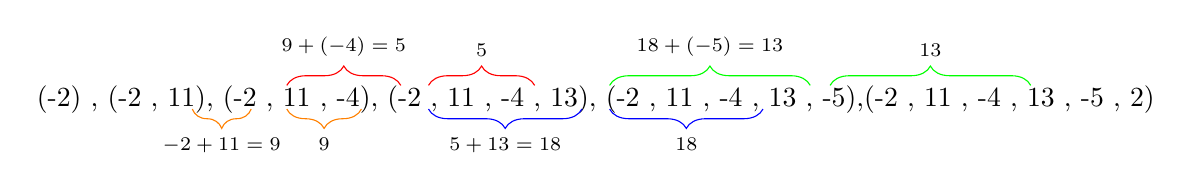
\begin{tikzpicture}[baseline]
    \node (A) at (0,0) {(-2) , (-2 , 11), (-2 , 11 , -4), (-2 , 11 , -4 , 13), (-2 , 11 , -4 , 13 , -5),(-2 , 11 , -4 , 13 , -5 , 2)};
 
    \node (X1) at (-5,0) {};
    \node (X2) at (-4.5,0) {};
    \node (X3) at (-3.8,0) {};
    \node (X4) at (-3.1,0) {};
    \node (Y1) at (-3.8,0.3) {};
    \node (Y2) at (-2.6,0.3) {};
    \node (Y3) at (-2,0.3) {};
    \node (Y4) at (-0.9,0.3) {};
    \node (Z1) at (-2,0) {};
    \node (Z2) at (-0.3,0) {};
    \node (Z3) at (0.3,0) {};
    \node (Z4) at (2,0) {};
    \node (A1) at (0.3,0.3) {};
    \node (A2) at (2.6,0.3) {};
    \node (A3) at (3.1,0.3) {};
    \node (A4) at (5.4,0.3) {};

    \draw [decorate, decoration={brace,amplitude=7pt,mirror}, orange]
        (X1.south west) -- (X2.south east) node[midway, below=7pt, black] {\scriptsize $-2+11 = 9$};
    \draw [decorate, decoration={brace,amplitude=7pt,mirror}, orange]
        (X3.south west) -- (X4.south east) node[midway, below=7pt, black] {\scriptsize $9$};
    \draw [decorate, decoration={brace,amplitude=7pt}, red]
        (Y1.south west) -- (Y2.south east) node[midway, above=7pt, black] {\scriptsize $9+(-4)=5$};
    \draw [decorate, decoration={brace,amplitude=7pt}, red]
        (Y3.south west) -- (Y4.south east) node[midway, above=7pt, black] {\scriptsize $5$};
    \draw [decorate, decoration={brace,amplitude=7pt,mirror}, blue]
        (Z1.south west) -- (Z2.south east) node[midway, below=7pt, black] {\scriptsize $5+13 = 18$};
    \draw [decorate, decoration={brace,amplitude=7pt,mirror}, blue]
        (Z3.south west) -- (Z4.south east) node[midway, below=7pt, black] {\scriptsize $18$};
    \draw [decorate, decoration={brace,amplitude=7pt}, green]
        (A1.south west) -- (A2.south east) node[midway, above=7pt, black] {\scriptsize $18+(-5)=13$};
    \draw [decorate, decoration={brace,amplitude=7pt}, green]
        (A3.south west) -- (A4.south east) node[midway, above=7pt, black] {\scriptsize $13$};

\end{tikzpicture}

\vspace{0.5em}

      \begin{itemize}[label={\tiny$\bullet$}]
        \item Nhận thấy, ta có thể tính tổng các phần tử từ vị trí $i$ đến $j$ từ tổng của các phần tử từ $i$ đến $j-1$ chỉ bằng 1 phép cộng:
      \end{itemize}

\vspace{-4em}

\color{HUSTRed}\large
        \[
        \sum_{k=i}^j a[k] = a[j] + \sum_{k=i}^{j-1} a[k]
        \]
  \begin{center}
    \vspace{-1em}
    \begin{tikzpicture}
    \node (X1) at (-4,0) {};
    \node (X2) at (-3,0) {};
    \node (X3) at (-1,0) {};
    \node (X4) at (-0,0) {};
        
    \draw [decorate, decoration={brace,amplitude=7pt,mirror}, blue]
        (X1.north west) -- (X2.north east) node[midway, below=7pt, black,xshift=-40pt] {\scriptsize Tổng các phần tử từ i đến j};
    \draw [decorate, decoration={brace,amplitude=7pt,mirror}, blue]
        (X3.north west) -- (X4.north east) node[midway, below=7pt, black,xshift=40pt] {\scriptsize Tổng các phần tử từ i đến j-1};
    \end{tikzpicture}
  \end{center}
\end{itemize}
\end{frame}

%slide 5 section 1
\begin{frame}[fragile]{1. Ví dụ minh họa}
  \color{HUSTRed}\large
        \[
        \sum_{k=i}^j a[k] = a[j] + \sum_{k=i}^{j-1} a[k]
        \]
  \begin{center}
    \begin{tikzpicture}
    \node (X1) at (-4,0) {};
    \node (X2) at (-3,0) {};
    \node (X3) at (-1,0) {};
    \node (X4) at (-0,0) {};
        
    \draw [decorate, decoration={brace,amplitude=7pt,mirror}, blue]
        (X1.north west) -- (X2.north east) node[midway, below=7pt, black,xshift=-40pt] {\scriptsize Tổng các phần tử từ i đến j};
    \draw [decorate, decoration={brace,amplitude=7pt,mirror}, blue]
        (X3.north west) -- (X4.north east) node[midway, below=7pt, black,xshift=40pt] {\scriptsize Tổng các phần tử từ i đến j-1};
    \end{tikzpicture}
  \end{center}
\vspace{-1em}
\begin{center}
\begin{tikzpicture}
  \node[inner sep=0pt] (box1) at (0,0) {
  % Node đầu là bảng code 1
    %C code1
    \begin{minipage}{0.42\textwidth}
        \begin{tcolorbox}[colback=gray!10, colframe=black, boxsep=0.1pt, left=0.1pt, right=0.1pt, top=0.1pt, bottom=0.1pt]
            \tiny
\begin{lstlisting}[language=C, basicstyle=\ttfamily\tiny\color{HUSTBlue}, breaklines=true ]
int maxSum = a[0];
for (int i=0; i<=n-1; i++) {
  for (int j=i; j<=n-1; j++) {
    int sum = 0;
    for (int k=i; k<=j; k++) sum += a[k];
    if (sum > maxSum) maxSum = sum;
  }
}
        \end{lstlisting}
      \end{tcolorbox}
    \end{minipage}
};

    %C code 2
    \node[inner sep=0pt] (box2) at (6.5,0) {
    \begin{minipage}{0.4\textwidth}
        \begin{tcolorbox}[colback=gray!10, colframe=black, boxsep=0.1pt, left=0.1pt, right=0.1pt, top=0.1pt, bottom=0.1pt]
            \tiny
\begin{lstlisting}[language=C, basicstyle=\ttfamily\tiny\color{HUSTBlue}, breaklines=true]
int maxSum = a[0];
for (int i=0; i<=n-1; i++) {
  int sum = 0;
  for (int j=i; j<=n-1; j++) {
    sum += a[j];
    if (sum > maxSum) maxSum = sum;
  }
}
        \end{lstlisting}
      \end{tcolorbox}
\end{minipage}
};
  \draw[line width=3mm ,-{Latex[length=8pt, width=14pt]}, orange] 
    ([xshift=0.05cm]box1.east)-- ([xshift=-0.05cm]box2.west);
\end{tikzpicture}
\end{center}
\end{frame}

\section{Một số khái niệm cơ bản về thuật toán}
\begin{frame}{2. Một số khái niệm cơ bản về thuật toán}
Nội dung slide
\begin{itemize}
  \item Nội dung 1
  \item Nội dung 2
  \item Nội dung 3
\end{itemize}
\end{frame}

\section{Ký hiệu tiệm cận}
\begin{frame}{3. Ký hiệu tiệm cận}
Nội dung slide
\begin{itemize}
  \item Nội dung 1
  \item Nội dung 2
  \item Nội dung 3
\end{itemize}
\end{frame}

\section{Kỹ thuật phân tích thuật toán}
\begin{frame}{4. Kỹ thuật phân tích thuật toán}
Nội dung slide
\begin{itemize}
  \item Nội dung 1
  \item Nội dung 2
  \item Nội dung 3
\end{itemize}
\end{frame}

{\HUSTUseBackground{theme_hust_oneside.pdf}
\begin{frame}
  \ifdefstring{\insertaspectratio}{169}{
    \placecontent{0.355\paperwidth}{0.410\paperheight}{0.640\paperwidth}{
        \color{HUSTRed}\bfseries\fontsize{28pt}{36pt}\selectfont\centering
        THANK YOU!
    }
  }{}
  \ifdefstring{\insertaspectratio}{43}{
    \placecontent{0.355\paperwidth}{0.440\paperheight}{0.640\paperwidth}{
        \color{HUSTRed}\bfseries\fontsize{28pt}{36pt}\selectfont\centering
        THANK YOU!
    }
  }{}
\end{frame}
}
{\HUSTUseBackground{theme_hust_oneside.pdf}
\begin{frame}
  \ifdefstring{\insertaspectratio}{169}{
    \placecontent{0.355\paperwidth}{0.320\paperheight}{0.640\paperwidth}{
        \color{HUSTRed}\bfseries\fontsize{28pt}{36pt}\selectfont\centering
        CẢM ƠN \\ĐÃ LẮNG NGHE!
    }
  }{}
  \ifdefstring{\insertaspectratio}{43}{
    \placecontent{0.355\paperwidth}{0.350\paperheight}{0.640\paperwidth}{
        \color{HUSTRed}\bfseries\fontsize{28pt}{36pt}\selectfont\centering
        CẢM ƠN \\ĐÃ LẮNG NGHE!
    }
  }{}
\end{frame}
}

\end{document}
